\section[Desenvolvimento do Projeto]{Desenvolvimento do Projeto}

\subsection{Repositório do Código Fonte do Projeto}
  Consultando outros colegas Ages 4, decidimos utilizar o GitHub como forma
primária de desenvolvimento, mantendo a versão do GitLab atualizada sempre por
meio de mirrors. Para gerar um mirror foi criado um token do GitLab com permissão
de modificar o conteúdo, a partir deste token criamos um workflow no GitHub Actions
que ao receber um push na main do GitHub replicava o push para o GitLab,
mantendo o GitLab sempre atualizado com a versão mais nova de produção.

  Para fins de manutenção do repositório e qualidade de código, utilizamos
proteções nas branches main e develop e seguimos a risca a definição do GitFlow,
que vale ressaltar foi um aprendizado de Gerenciamento e Configuração de
Software, que provou-se muito útil mesmo ao passar do tempo com matérias mais
complexas entrando.

  Por fim dispomos do padrão de commits Conventional Commits para garantir
que o repositório tenha os commits padronizados e mais fáceis de entender,
garantindo seu uso através de ferramentas como Husky no Frontend e Pre Commit
no Backend. Além disso foram usados linters e formatadores para garantir que o
código seguisse um padrão de qualidade e padronização mínimo, facilitando o
trabalho de quem revisasse os pull requests. No Fronted a tarefa de linting ficou com
o ESLint e a formatação com o Prettier, enquanto no Backend uma ferramenta nova
pelo nome de Ruff entregou resultados em ambas as tarefas ao mesmo tempo que
se manteve performático enquanto rodava em background.

Back-end: \urlref{https://tools.ages.pucrs.br/vango/vango-api}
Front-end: \urlref{https://tools.ages.pucrs.br/vango/vango-frontend}

\subsection{Banco de Dados Utilizado}
  Quanto ao banco de dados, ficamos em dúvida entre o relacional e o não-
relacional, a princípio a escolha do relacional conversava muito bem com o escopo
definido que planejavamos ter, no entanto, utilizando Python e até considerando
utilizar serviços do Firebase, ficamos muito inclinados no começo a utilizar um banco
de dados não-relacional, seja ele um MongoDB pela fácil integração com Python ou
o Cloud Firestore do Firebase pela facilidade da nuvem e o atrito inicial quebrado
pelo fato do time já ter criado uma conta do Firebase.

  Ainda assim, pela naturalidade dos tipos de dados que tinhamos e a
capacidade como planejamos trabalhar com um escopo definido e relações bem
claras entre entidades, decidimos por utilizar um banco relacional. A partir disto
tinhamos que decidir entre as opções disponíveis no mercado, a primeira ideia é
sempre o PostgreSQL, visto a modernidade e ascensão recente do banco, devido ao
suporte a JSON e outras features avançadas. O domínio do PostgreSQL também
pode ser visto nas pesquisas de desenvolvedores do StackOverflow de 2025, onde
por mais um ano, continua na liderança em adesão geral e principalmente em
adesão por profissionais.

  Os motivos anteriores já seriam o bastante para justificar a escolha deste
Sistema Gerenciador de Banco de Dados, no entanto, pesquisando mais a fundo
encontramos motivos mais válidos ainda para consolidar nossa escolha. Elencamos
como um bônus um banco que pudesse trabalhar de maneira performática com
geolocalização, visto que essa parece ser uma das prioridades dos stakeholders
para quando o desenvolvimento passar para eles. Sendo assim achamos uma
extensão de Postgres, chamada PostGIS que permite o uso de campos de latitude e
longitude que se comportam de forma otimizada, permitindo essa fácil migração no
caso da necessidade de melhorar a performance no futuro.

\begin{figure}[H]
    \centering
    \small
    \caption{Time do Projeto VanGO}
    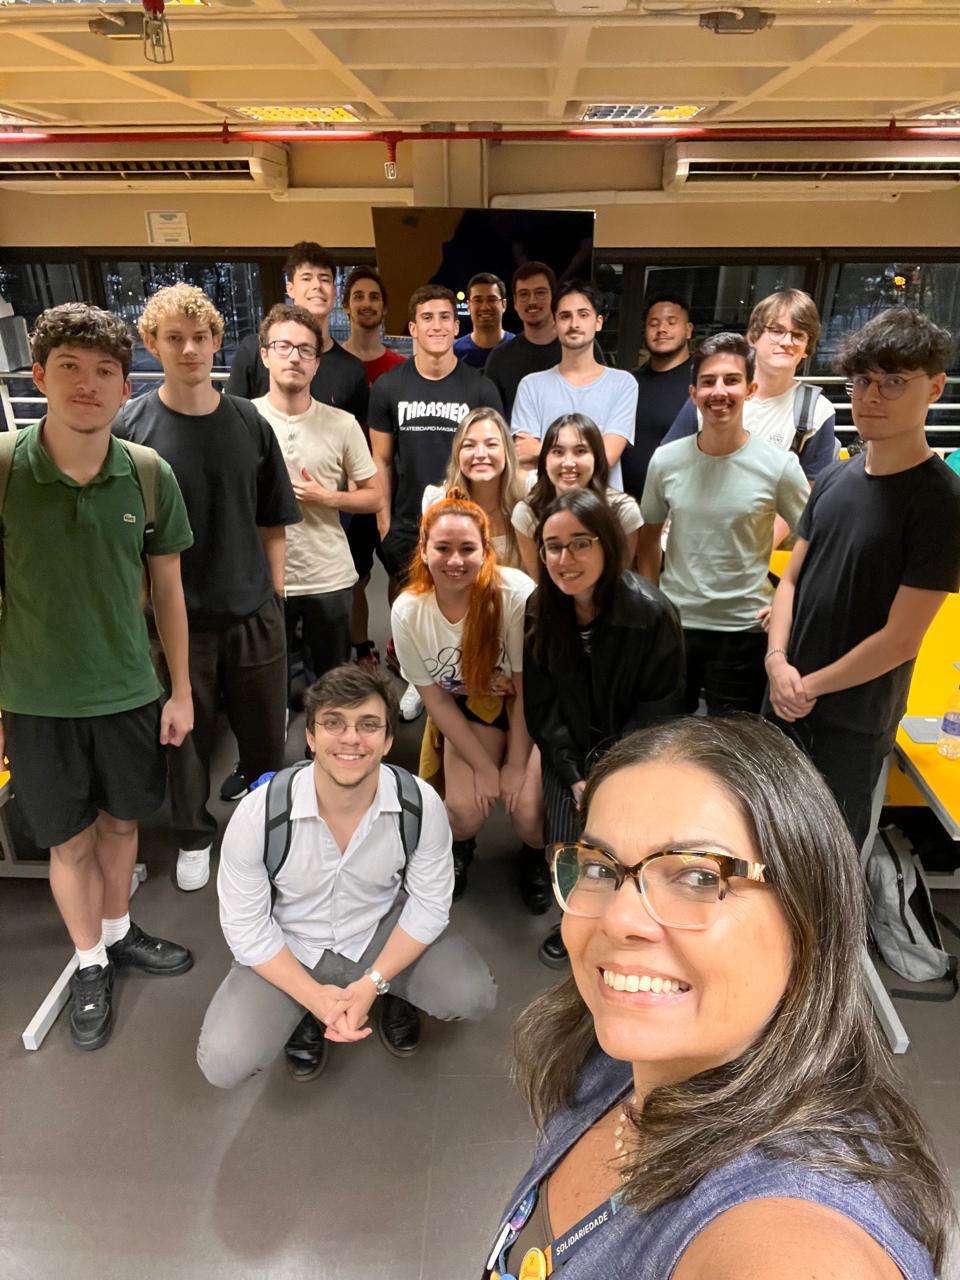
\includegraphics[width=1\linewidth]{conteudo//4 - ages III//conteudo//figures/vango-time.png}
    Fonte: Wiki do Projeto
    \label{fig:projeto-time-vango}
\end{figure}

  Na modelagem destaca-se a presença de rastreabilidade em quase todas as
tabelas, com a presença dos campos \texttt{created\_at} e \texttt{updated\_at}, na maioria das
entidades que permitem criação e edição por parte do usuário. Além disso campos
interessantes são o de \texttt{photo\_url} que é usado para sincronizar com o bucket que
guarda os uploads e o \texttt{password\_hash} que possui um nome bem descritivo,
ressaltando o uso da biblioteca bcrypt na criptografia da senha do usuário.
Banco de Dados: \urlref{https://tools.ages.pucrs.br/vango/vango-wiki/-/wikis/database}

\subsection{Arquitetura Utilizada}
  Utilizamos um divisão clara de arquitetura entre Backend e Frontend. No
Backend optamos por um híbrido de Clean Architecture com Camadas, a ideia foi ter
a testabilidade e o desacoplamento fornecido por uma Clean Architecture, sem o
overheading que ela muitas vezes é criticada por trazer ao projeto. Na prática, do
service para frente tudo é abstraído, já antes dele é utilizada uma arquitetura de
camadas para não sobrecarregar os programadores novatos com UseCases e
Mappers.

  A imagem abaixo representa muito bem o diagrama de uma feature do
sistema, a de criar usuário, incluindo a interação com a criptografia e como fizemos
para abstrair essa parte de hashing. Note que segundo pesquisas dos integrantes da
equipe, pelo fato do Python não possuir um jeito opinativo de injeção de
dependências, o método mais adequado é o uso da classe UserDependencies.

\begin{figure}[H]
    \centering
    \small
    \caption{Time do Projeto VanGO}
    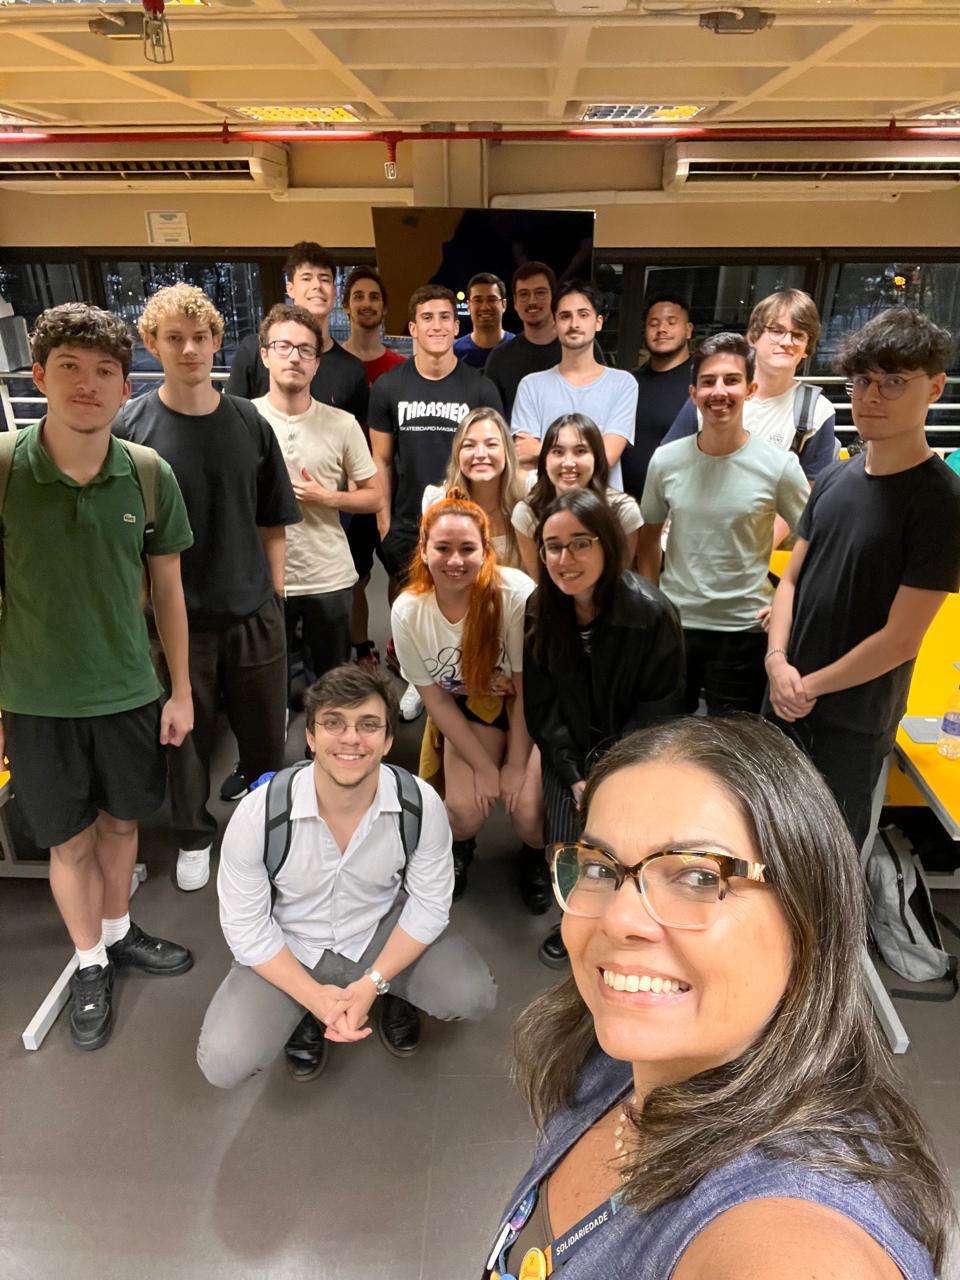
\includegraphics[width=1\linewidth]{conteudo//4 - ages III//conteudo//figures/vango-time.png}
    Fonte: Wiki do Projeto
    \label{fig:projeto-time-vango}
\end{figure}

  Já no Frontend conseguimos ver uma separação de camadas, que isola em
arquivos diferentes Layout, Hooks, Services e API. Esse isolamento permite uma
arquitetura híbrida, onde Services e API, falam a mesma linguagem do Backend,
agindo de maneira orientada a domínio, enquanto Layout e Hooks, conversam de
maneira orientada aos casos de uso da aplicação do Frontend. Sendo assim a
tradução ocorre entre as camadas de Hooks e Services.

  Podemos observar na imagem abaixo a retratação de uma feature simples do
Frontend, a de criar dependente. Vale notar o modo como a arquitetura integra
ferramentas como TanStack, zod e react-hook-form com a arquitetura base para
garantir maior confiabilidade, validação e principlamente o uso devido da cache
entregando melhor performance. Vale notar também a centralização do Design
System visível na pasta styles, responsável por especificar cores e tipografias para
garantir a padronização ao redor do código.

\begin{figure}[H]
    \centering
    \small
    \caption{Time do Projeto VanGO}
    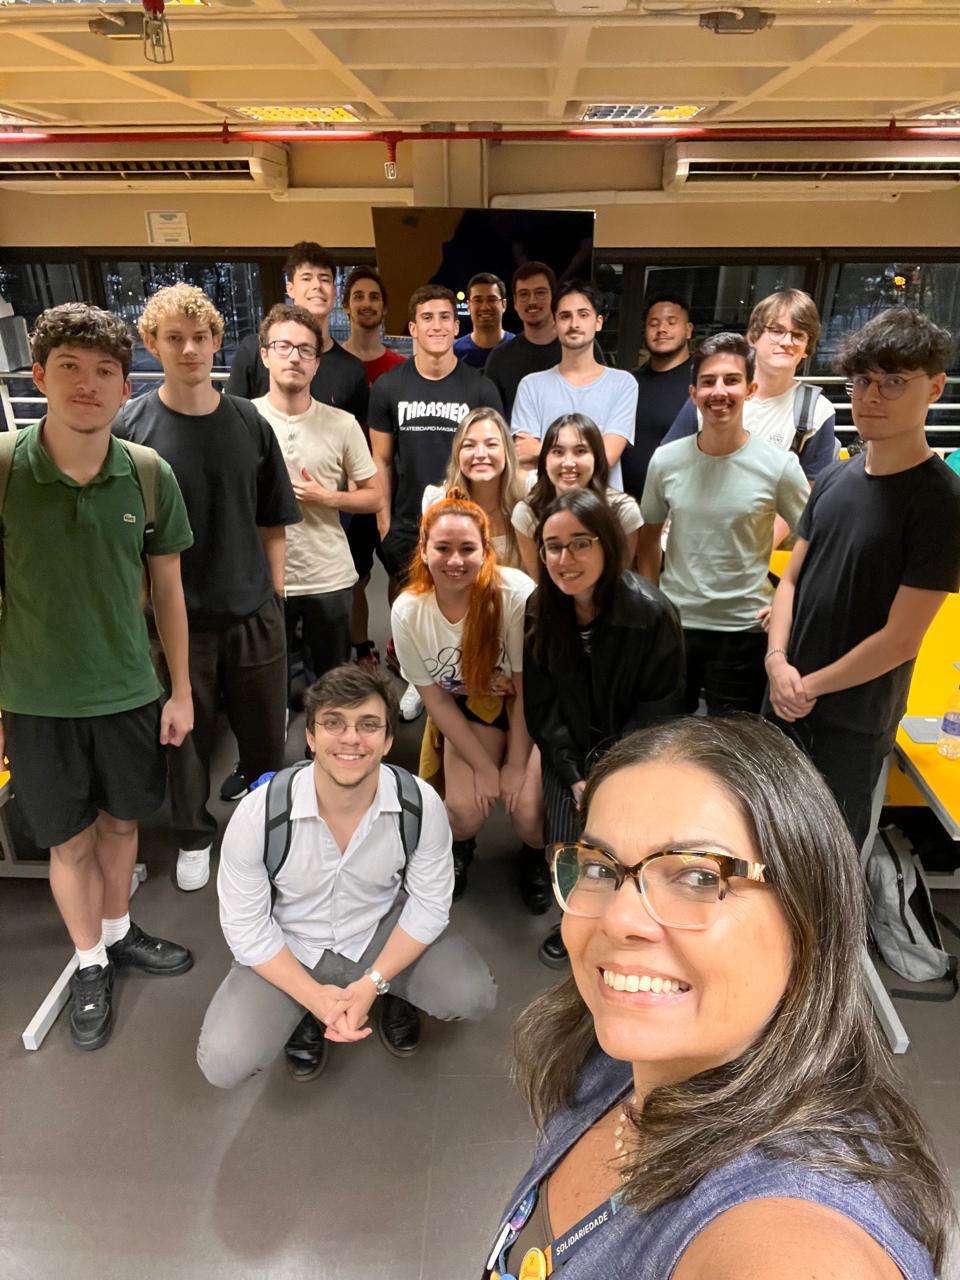
\includegraphics[width=1\linewidth]{conteudo//4 - ages III//conteudo//figures/vango-time.png}
    Fonte: Wiki do Projeto
    \label{fig:projeto-time-vango}
\end{figure}

Arquitetura: https://tools.ages.pucrs.br/vango/vango-wiki/-/wikis/arquitetura

\subsection{Protótipos das Telas Desenvolvidas}
  Utilizamos a ferramenta Figma para a prototipação das telas do usuário.
Aproveitamos da proficiência de algumas integrantes do grupo nesta ferramenta,
com a vontade de aprender dos mais novatos para entregar diversas telas
padronizadas, seguindo um Design System costumizado e muito bem escolhido.

  Escolhemos o uso da cor amarela e especficamente nesta tonalidade a
pedido dos stakeholders que especificaram o desejo de adotar na identidade visual a
cor amarela na tonalidade presente nas vans escolares. Junto a isso, trouxemos a
cor azul escura como um complementar à cor amarela escolhida e o branco para
uma tonalidade mais neutra e limpa, além de algumas outras cores complementares,
como podemos ver na imagem abaixo.

\begin{figure}[H]
    \centering
    \small
    \caption{Time do Projeto VanGO}
    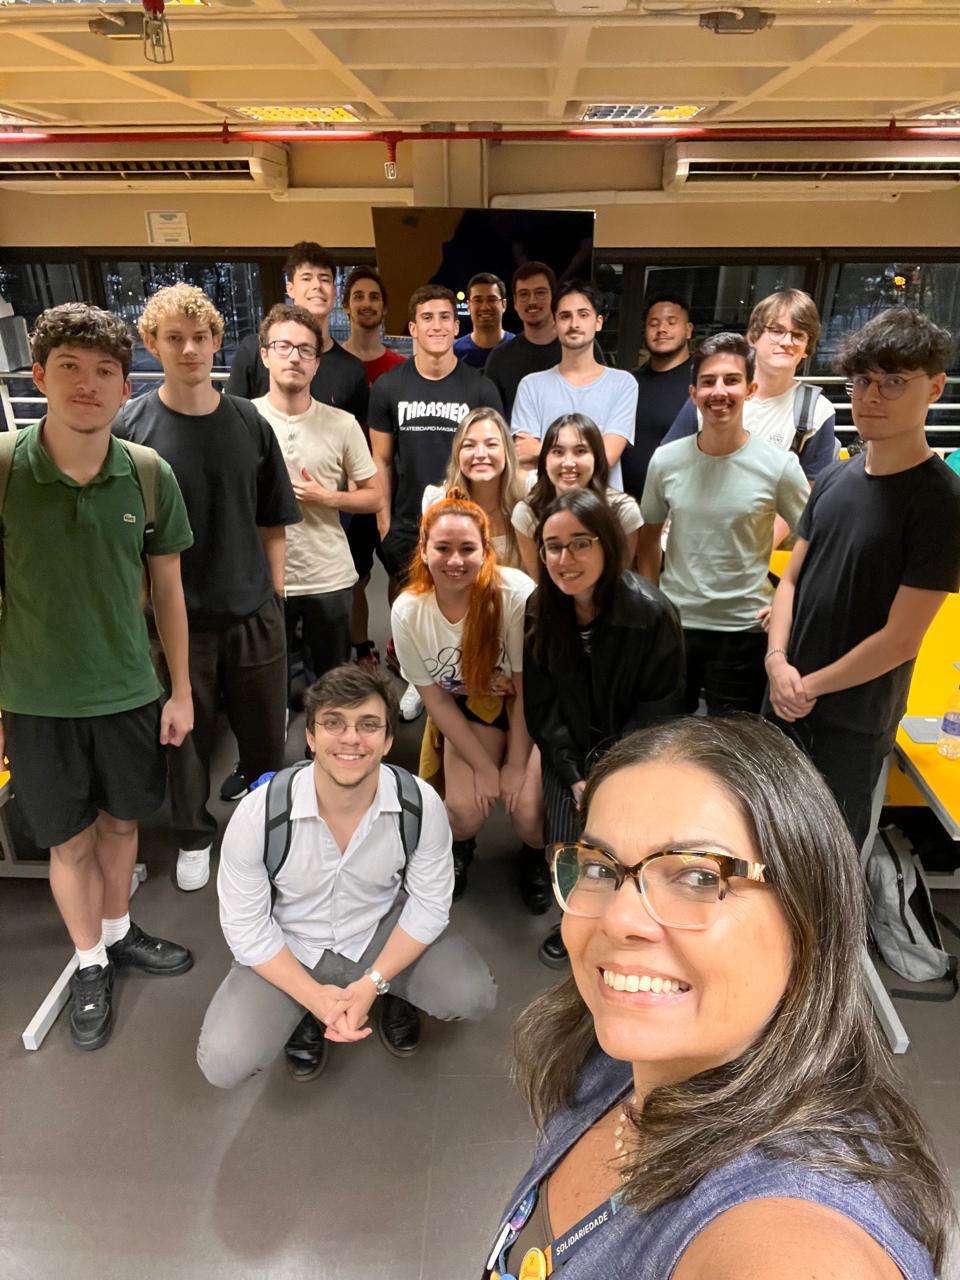
\includegraphics[width=1\linewidth]{conteudo//4 - ages III//conteudo//figures/vango-time.png}
    Fonte: Wiki do Projeto
    \label{fig:projeto-time-vango}
\end{figure}

  A prototipação conta com cerca de 50 telas diferentes, portanto, haverá uma
abstração, mostrando apenas as telas mais importantes ou que tenham a lógica
mais complexa de implementação. No entanto, caso queira conferir todas as telas ao
final dessa seção haverá um link.

\begin{figure}[H]
    \centering
    \small
    \caption{Time do Projeto VanGO}
    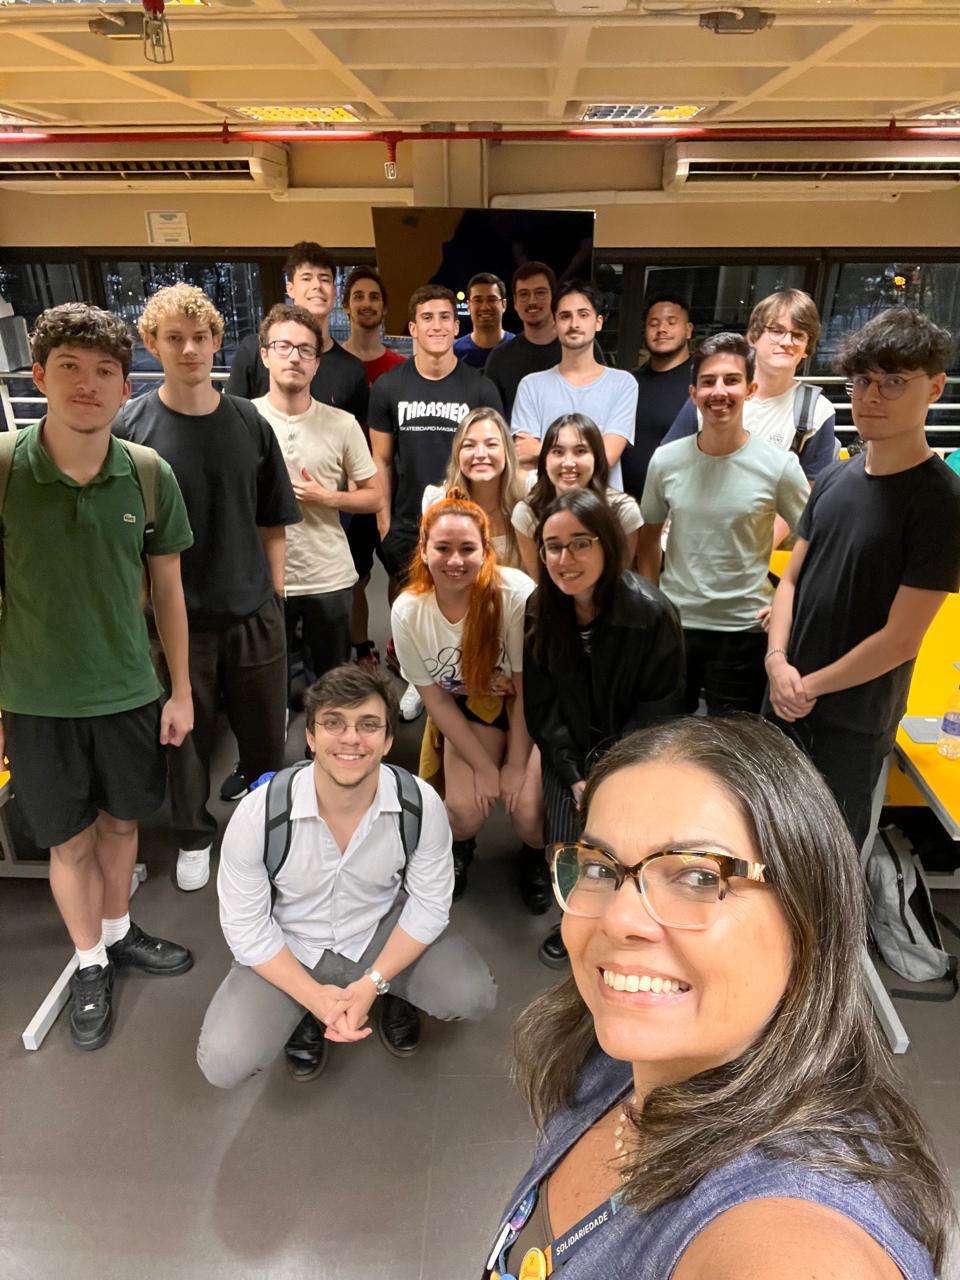
\includegraphics[width=1\linewidth]{conteudo//4 - ages III//conteudo//figures/vango-time.png}
    Fonte: Wiki do Projeto
    \label{fig:projeto-time-vango}
\end{figure}

\begin{figure}[H]
    \centering
    \small
    \caption{Time do Projeto VanGO}
    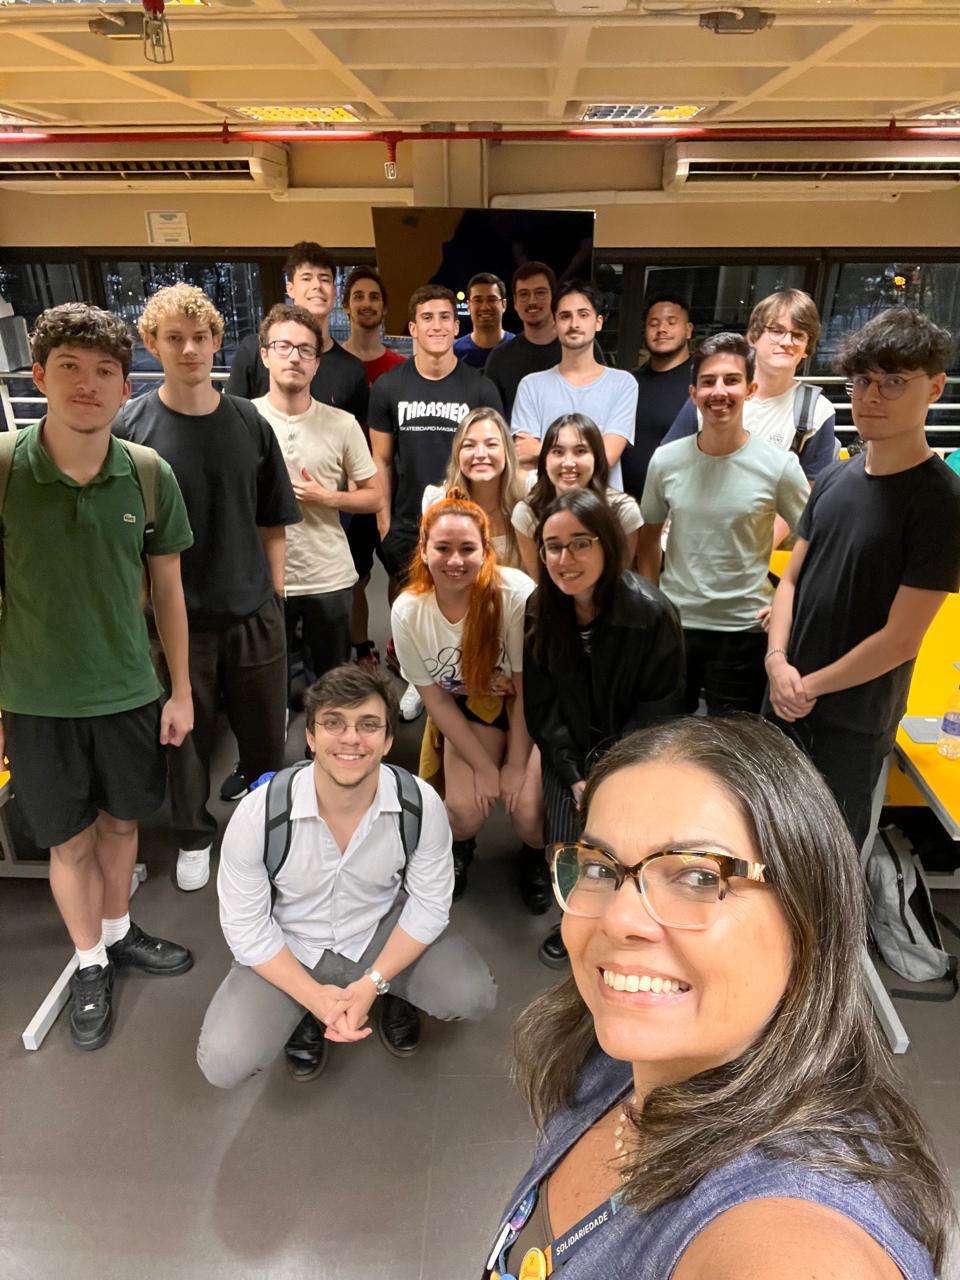
\includegraphics[width=1\linewidth]{conteudo//4 - ages III//conteudo//figures/vango-time.png}
    Fonte: Wiki do Projeto
    \label{fig:projeto-time-vango}
\end{figure}

\begin{figure}[H]
    \centering
    \small
    \caption{Time do Projeto VanGO}
    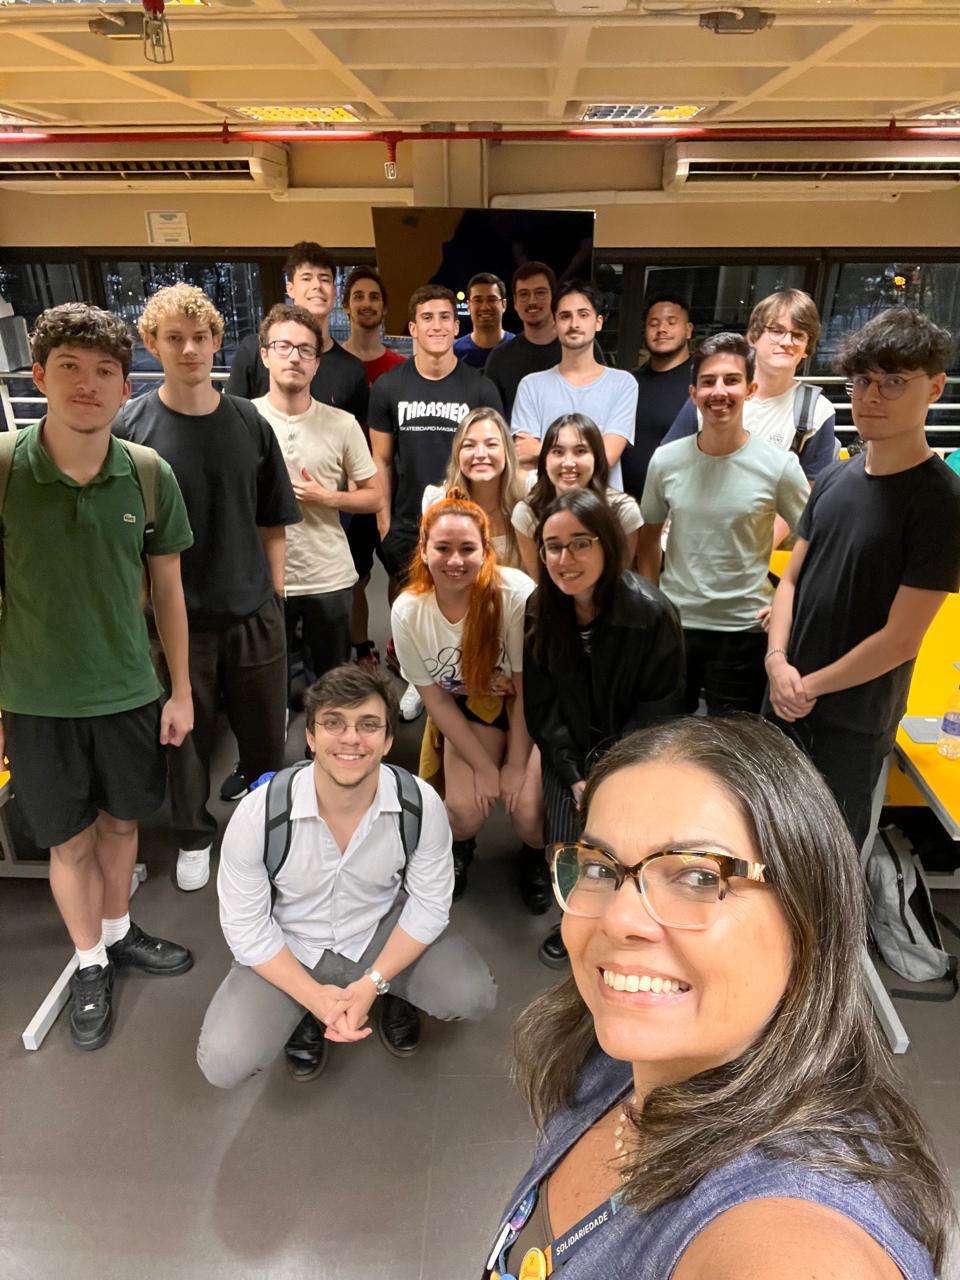
\includegraphics[width=1\linewidth]{conteudo//4 - ages III//conteudo//figures/vango-time.png}
    Fonte: Wiki do Projeto
    \label{fig:projeto-time-vango}
\end{figure}

Mockups: https://tools.ages.pucrs.br/vango/vango-wiki/-/wikis/mockups

\subsection{Tecnologias Utilizadas}
  
  Após realizarmos uma pesquisa com os novatos, principalmente para definir
linguagem de Backend que eles tinham familiaridade, o Python surgiu como um forte
candidato, perdendo apenas para o Java devido ao posterior ser ensinado por
padrão no currículo atual da PUCRS. Ainda assim, visando integrações mais
complexas que desejávamos fazer a escolha de Python parecia óbvia e se fez mais
ainda a partir do momento que validamos o uso da linguagem com o stakeholder.

  Quanto ao framework, tinhamos uma escolha entre Django, Flask e FastAPI,
na qual a maioria dominava melhor o FastAPI e apesar da minha insatisfação parcial
com a tecnologia, visto que minha última experiência com o FastAPI que foi a Ages
2 deixou um pouco a desejar, fui voto vencido e portanto tive que seguir no FastAPI,
até pensando em um senso de coletividade e trabalho em equipe creio que foi a
melhor decisão mesmo.

  Além disso tinhamos outras decisões relacionadas a ORM e versionamento
de migrations, para as quais fizemos uma boa pesquisa. No que diz respeito ao
ORM escolhemos o SQLAlchemy, mesmo tendo uma experiência negativa com ele
em meu projeto passado, resolvi dar uma nova chance, tendo em vista que a
tecnologia deve estar mais madura atualmente, tendo em vista que o mesmo lançou
muito perto da data daquela Ages e portanto ainda faltavam features e a
documentação ainda pecava um pouco.

  Já para migrations o Alembic se mostrou uma das melhores opções
permitindo uma combinação de customização com facilidade de entrada, permitindo
que se gerasse as primeiras migrations sem nenhuma barreira de entrada, ao
mesmo tempo que permite modificar totalmente como elas são geradas em um
arquivo do Alembic.

  Quanto ao Frontend, utilizamos a linguagem TypeScript com a biblioteca
React Native e o framework Expo. Além disso ferramentas como TanStack para
controlar cache e outras funcionalidades, Zustand para gerenciamento de estado
global, Zod para validar formulários e outros.